\section{Конструкторская часть}

В этом разделе будут представлены схемы и/или псевдокоды реализуемых алгоритмов.

\subsection{Требования к ПО}
К программе предъявляется ряд требований:
\begin{itemize}[]
	\item искомая подстрока имеет размер $S$ от 6 до 10 символов;
	\item первые две пары символов искомой подстроки совпадают;
	\item при генерации исходной строки шанс 7/8 сгенерировать подстроку из $S$ случайных символов;
	\item при генерации исходной строки шанс 1/8 сгенерировать искомую подстроку, конкотенирующую с её первой парой символов, т.е. получить подстроку длины $S + 2$ символов;
	\item на вход подается строка и искомая в ней подстрока;
	\item на выходе требуется получить файл с записями индексов вхождения подстроки.
	
\end{itemize}

\newpage
\subsection{Разработка алгоритмов}

В листинге~\ref{alg:standart} рассмотрен псевдокод стандартного алгоритма поиска подстроки в строке.

\begin{algorithm}[H]
	\caption{Стандартный алгоритм}
	\label{alg:standart}
	\SetAlgoLined
	\KwIn{Строка $text$, подстрока $pattern$}
	\KwOut{Индекс первого вхождения $pattern$ в $text$, или -1 если не найден}
	$n \gets \text{length}(text)$\;
	$m \gets \text{length}(pattern)$\;
	\For{$i \gets 1$ \KwTo $n - m + 1$}{
		$j \gets 1$\;
		\While{$j \leq m$ \textbf{and} $text[i + j - 1] = pattern[j]$}{
			$j \gets j + 1$\;
		}
		\If{$j > m$}{
			\KwRet{$i$}\;
		}
	}
	\KwRet{-1}\;
\end{algorithm}

\newpage

Алгоритм Кнута-Морриса-Пратта поиска подстроки в строке использует префиксную функцию. 
Префиксная функция, вычисляемая для искомой подстроки, содержит сведения о том, в какой мере образец совпадает сам с собой после сдвигов. 
Эта информация помогает избежать лишних проверок при поиске~\cite{алексеенко2010информационная}.

В листинге~\ref{alg:pre} рассмотрен псевдокод алгоритма расчета префиксного массива.

\begin{algorithm}[H]
	\caption{Расчет префиксного массива}
	\label{alg:pre}
	\SetAlgoLined
	\KwIn{Подстрока $x$}
	\KwOut{Префиксный массив $\pi$}
	$m \gets \text{length}(x)$\;
	$\pi[0] \gets 0$\;
	$k \gets 0$\;
	\For{$q \gets 1$ \KwTo $m$}{
		\While{$k > 0$ \textbf{и} $x[k + 1] \neq x[q]$}{
			$k \gets \pi[k]$\;
		}
		\If{$x[k + 1] = x[q]$}{
			$k \gets k + 1$\;
		}
		$\pi[q] \gets k$\;
	}
	\KwRet{$\pi$}\;
\end{algorithm}

\newpage
В листинге~\ref{alg:kmp} рассмотрен псевдокод алгоритма Кнута~--~Морриса~--~Пратта.

\begin{algorithm}[H]
	\caption{Кнута~--~Морриса~--~Пратта}
	\label{alg:kmp}
	\SetAlgoLined
	\KwIn{Строка $w = a_1 \dots a_n$, подстрока $x = b_1 \dots b_m$, префиксный массив $\pi$}
	$i \gets 0$\;
	$j \gets 0$\;
	$n \gets \text{length}(w)$\;
	$m \gets \text{length}(x)$\;
	\While{$i < n$}{
		\If{$a_i = b_j$}{
			$i \gets i + 1$\;
			$j \gets j + 1$\;
			\If{$j = m$}{
				\KwRet{$i - n$}\;
			}
		}
		\Else{
			\If{$j = 0$}{
				$i \gets i + 1$\;
			}
			\Else{
				$j \gets \pi[j - 1]$\;
			}
		}
	}
	\KwRet{$-1$}\;
\end{algorithm}
\newpage

На рисунке \ref{fig:linear} изображен последовательный случай реализации конвейера.

\begin{figure}
	\centering
	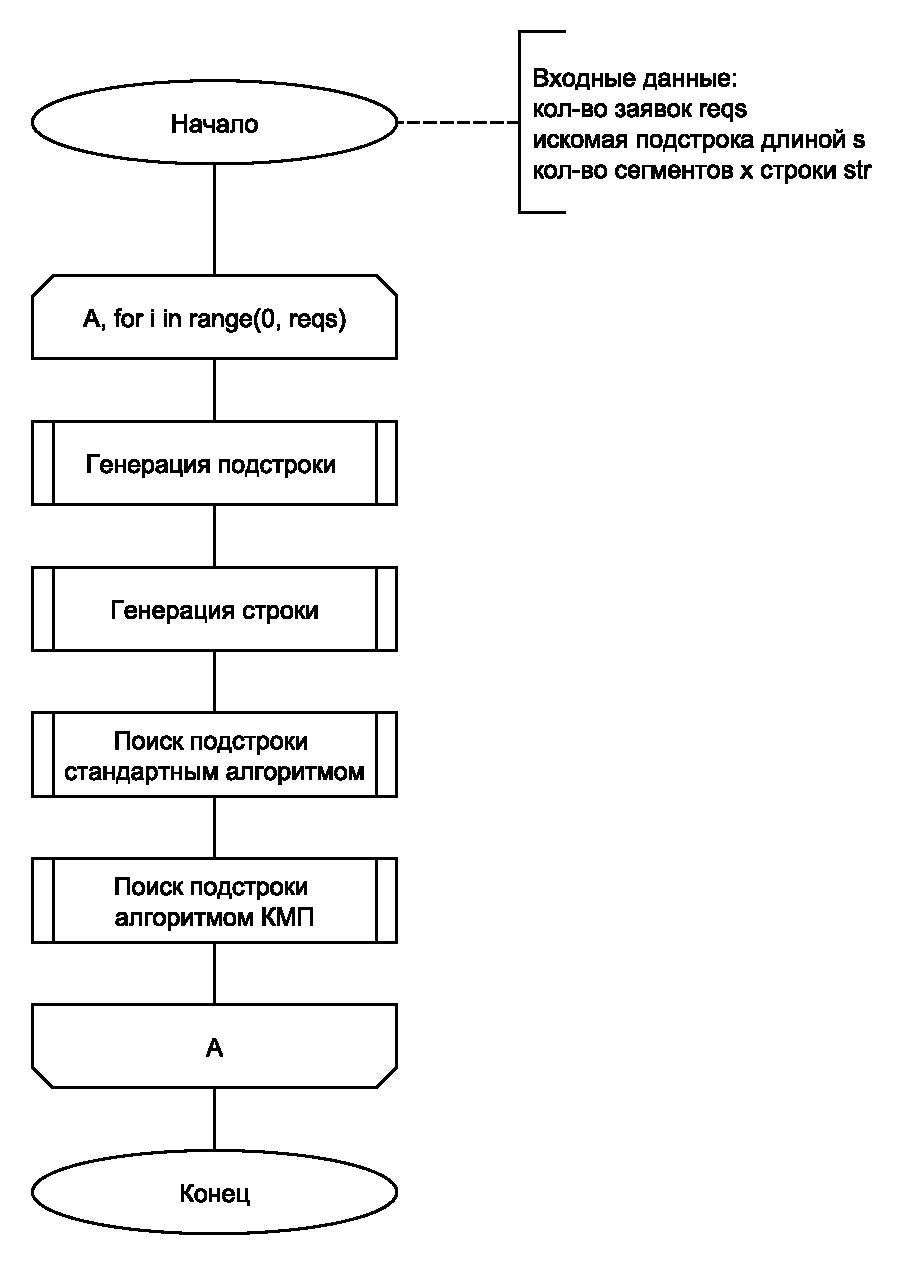
\includegraphics[width=0.7\linewidth]{images/linear}
	\caption[Последовательная обработка лент]{}
	\label{fig:linear}
\end{figure}

На рисунке \ref{fig:parallel} изображен параллельный случай реализации конвейера.
Он заключается в том, что все вторая и третья ленты выполняются одновременно в разных потоках.

\begin{figure}
	\centering
	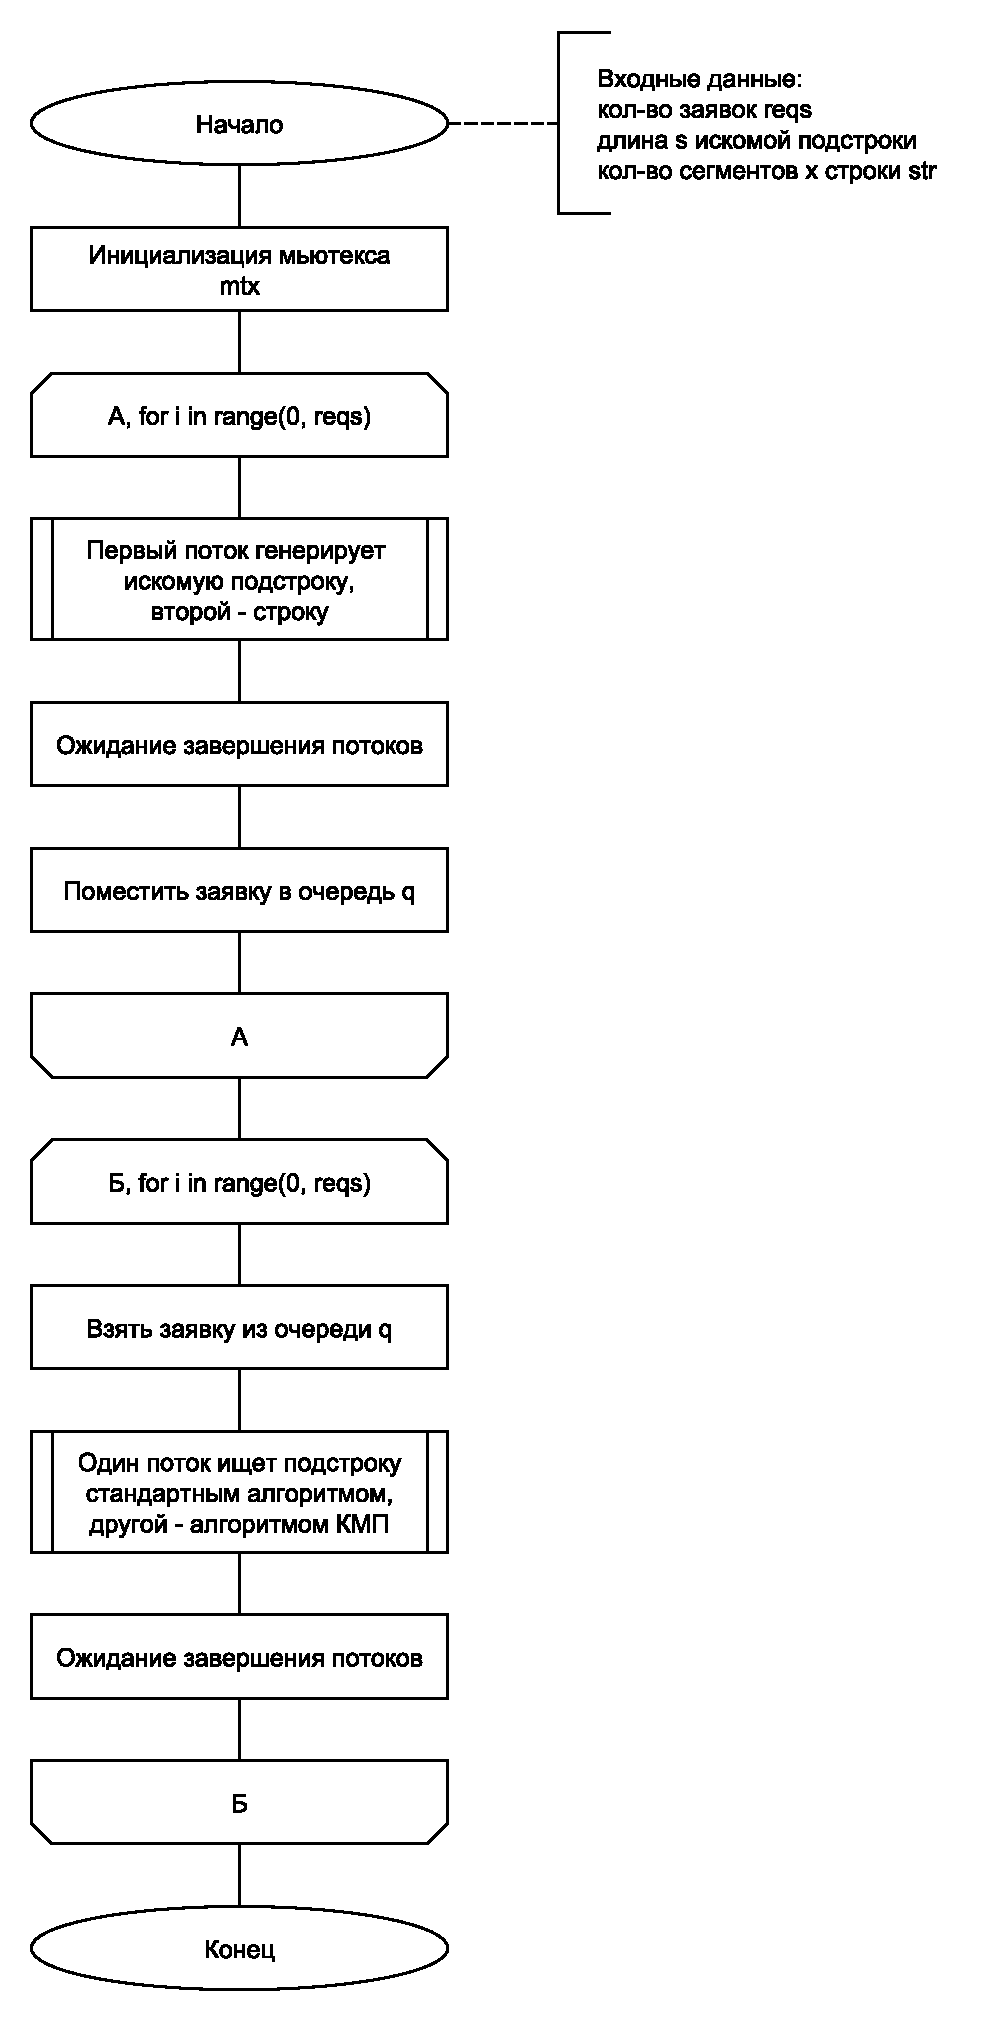
\includegraphics[width=0.7\linewidth]{images/parallel}
	\caption[Параллельная конвейерная обработка]{}
	\label{fig:parallel}
\end{figure}

При этом, функция записи лога на рисунке~\ref{fig:log} содержит критическую секцию, доступ к которой ограничивается мьютексом, который передается каждому потоку.

\begin{figure}
	\centering
	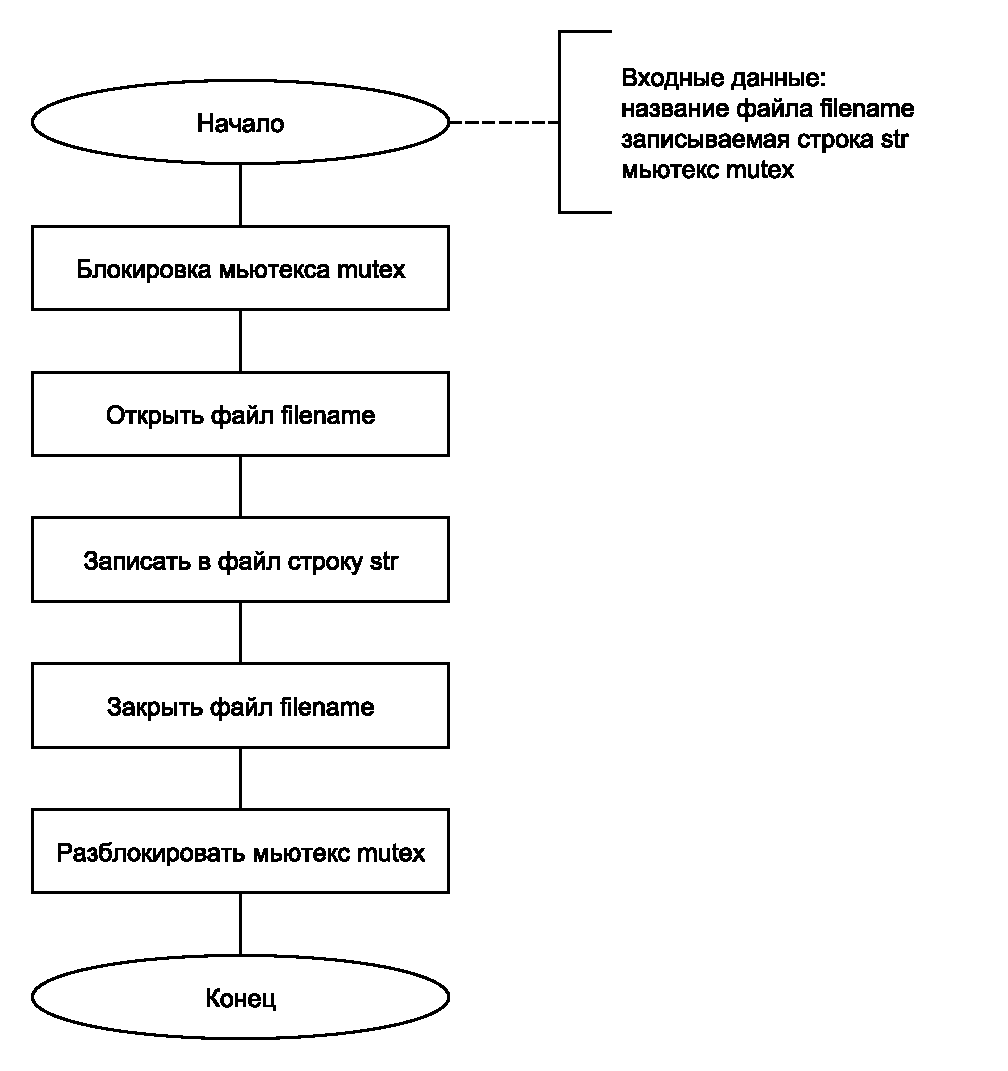
\includegraphics[width=0.7\linewidth]{images/log.pdf}
	\caption[Запись строки в файл]{}
	\label{fig:log}
\end{figure}